% arara: pdflatex
% arara: pdflatex
% arara: pdflatex

% options:
% thesis=B bachelor's thesis
% thesis=M master's thesis
% czech thesis in Czech language
% slovak thesis in Slovak language
% english thesis in English language
% hidelinks remove colour boxes around hyperlinks

\documentclass[thesis=B,english]{FITthesis}[2019/12/23]

\usepackage[utf8]{inputenc} % LaTeX source encoded as UTF-8

% \usepackage{amsmath} %advanced maths
% \usepackage{amssymb} %additional math symbols

\usepackage{dirtree} %directory tree visualisation

% % list of acronyms
% \usepackage[acronym,nonumberlist,toc,numberedsection=autolabel]{glossaries}
% \iflanguage{czech}{\renewcommand*{\acronymname}{Seznam pou{\v z}it{\' y}ch zkratek}}{}
% \makeglossaries

\newcommand{\tg}{\mathop{\mathrm{tg}}} %cesky tangens
\newcommand{\cotg}{\mathop{\mathrm{cotg}}} %cesky cotangens

% % % % % % % % % % % % % % % % % % % % % % % % % % % % % % 
% ODTUD DAL VSE ZMENTE
% % % % % % % % % % % % % % % % % % % % % % % % % % % % % % 

\department{Department of Software Engineering}
\title{Mobile client for LinkedPipes ETL on the Android platform}
\authorGN{David} %(křestní) jméno (jména) autora
\authorFN{Paleček} %příjmení autora
\authorWithDegrees{David Paleček} %jméno autora včetně současných akademických titulů
\author{David Paleček} %jméno autora bez akademických titulů
\supervisor{RNDr. Jakub Klímek, Ph.D.}
%\acknowledgements{Doplňte, máte-li komu a za co děkovat. V~opačném případě úplně odstraňte tento příkaz.}
\abstractCS{Tato práce se zabývá tvorbou androidového klienta pro LinkedPipes ETL. Obsahuje všechny stádia vývoje této aplikace.}
\abstractEN{This work deals with the creation of an Android client for LinkedPipes ETL. It contains all stages of development of this application.}
\placeForDeclarationOfAuthenticity{V~Praze}
\declarationOfAuthenticityOption{4} %volba Prohlášení (číslo 1-6)
\keywordsCS{android, klient, linked, pipes, etl}
\keywordsEN{android, client, linked, pipes, etl}
% \website{http://site.example/thesis} %volitelná URL práce, objeví se v tiráži - úplně odstraňte, nemáte-li URL práce
\usepackage{pdfpages}
\begin{document}

% \newacronym{CVUT}{{\v C}VUT}{{\v C}esk{\' e} vysok{\' e} u{\v c}en{\' i} technick{\' e} v Praze}
% \newacronym{FIT}{FIT}{Fakulta informa{\v c}n{\' i}ch technologi{\' i}}

\begin{introduction}
	%sem napište úvod Vaší práce
	//TODO
\end{introduction}

%\chapter{Work goal}
%The goal of this thesis is to pitch an Android client for the \etl{} system as an alternative to opening a web page in a mobile browser.

In order to do that, following steps must be fulfilled.

\begin{itemize}
    \item A list of requirements for the application will be put together in the analysis chapter.
    \item Existence of no current solution will be verified in the existing solutions chapter.
    \item Application will be designed, including appearance and code layering, in the design chapters.
    \item Result of the implementation chapter will be the application.
    \item Documentation will be created after the application is created and described in the documentation chapter.
    \item Application tests will be described in the test chapter.
\end{itemize}
%
%%% % % % % % % % % % % % % % % % % % % % % % % % % % % % 
% Tuto kapitolu z výsledné práce ODSTRAŇTE.
% % % % % % % % % % % % % % % % % % % % % % % % % % % 

\chapter{Návod k~použití této šablony}

Tento dokument slouží jako základ pro napsání závěrečné práce na Fakultě informačních technologií ČVUT v~Praze.

\section{Výběr základu}

Vyberte si šablonu podle druhu práce (bakalářská, diplomová), jazyka (čeština, angličtina) a kódování (ASCII, \mbox{UTF-8}, \mbox{ISO-8859-2} neboli latin2 a nebo \mbox{Windows-1250}). 

V~české variantě naleznete šablony v~souborech pojmenovaných ve formátu práce\_kódování.tex. Typ může být:
\begin{description}
	\item[BP] bakalářská práce,
	\item[DP] diplomová (magisterská) práce.
\end{description}
Kódování, ve kterém chcete psát, může být:
\begin{description}
	\item[UTF-8] kódování Unicode,
	\item[ISO-8859-2] latin2,
	\item[Windows-1250] znaková sada 1250 Windows.
\end{description}
V~případě nejistoty ohledně kódování doporučujeme následující postup:
\begin{enumerate}
	\item Otevřete šablony pro kódování UTF-8 v~editoru prostého textu, který chcete pro psaní práce použít -- pokud můžete texty s~diakritikou normálně přečíst, použijte tuto šablonu.
	\item V~opačném případě postupujte dále podle toho, jaký operační systém používáte:
	\begin{itemize}
		\item v~případě Windows použijte šablonu pro kódování \mbox{Windows-1250},
		\item jinak zkuste použít šablonu pro kódování \mbox{ISO-8859-2}.
	\end{itemize}
\end{enumerate}


V~anglické variantě jsou šablony pojmenované podle typu práce, možnosti jsou:
\begin{description}
	\item[bachelors] bakalářská práce,
	\item[masters] diplomová (magisterská) práce.
\end{description}

\section{Použití šablony}

Šablona je určena pro zpracování systémem \LaTeXe{}. Text je možné psát v~textovém editoru jako prostý text, lze však také využít specializovaný editor pro \LaTeX{}, např. Kile.

Pro získání tisknutelného výstupu z~takto vytvořeného souboru použijte příkaz \verb|pdflatex|, kterému předáte cestu k~souboru jako parametr. Vhodný editor pro \LaTeX{} toto udělá za Vás. \verb|pdfcslatex| ani \verb|cslatex| \emph{nebudou} s~těmito šablonami fungovat.

Více informací o~použití systému \LaTeX{} najdete např. v~\cite{wikilatex}.

\subsection{Typografie}

Při psaní dodržujte typografické konvence zvoleného jazyka. České \uv{uvozovky} zapisujte použitím příkazu \verb|\uv|, kterému v~parametru předáte text, jenž má být v~uvozovkách. Anglické otevírací uvozovky se v~\LaTeX{}u zadávají jako dva zpětné apostrofy, uzavírací uvozovky jako dva apostrofy. Často chybně uváděný symbol "{} (palce) nemá s~uvozovkami nic společného.

Dále je třeba zabránit zalomení řádky mezi některými slovy, v~češtině např. za jednopísmennými předložkami a spojkami (vyjma \uv{a}). To docílíte vložením pružné nezalomitelné mezery -- znakem \texttt{\textasciitilde}. V~tomto případě to není třeba dělat ručně, lze použít program \verb|vlna|.

Více o~typografii viz \cite{kobltypo}.

\subsection{Obrázky}

Pro umožnění vkládání obrázků je vhodné použít balíček \verb|graphicx|, samotné vložení se provede příkazem \verb|\includegraphics|. Takto je možné vkládat obrázky ve formátu PDF, PNG a JPEG jestliže používáte pdf\LaTeX{} nebo ve formátu EPS jestliže používáte \LaTeX{}. Doporučujeme preferovat vektorové obrázky před rastrovými (vyjma fotografií).

\subsubsection{Získání vhodného formátu}

Pro získání vektorových formátů PDF nebo EPS z~jiných lze použít některý z~vektorových grafických editorů. Pro převod rastrového obrázku na vektorový lze použít rasterizaci, kterou mnohé editory zvládají (např. Inkscape). Pro konverze lze použít též nástroje pro dávkové zpracování běžně dodávané s~\LaTeX{}em, např. \verb|epstopdf|.

\subsubsection{Plovoucí prostředí}

Příkazem \verb|\includegraphics| lze obrázky vkládat přímo, doporučujeme však použít plovoucí prostředí, konkrétně \verb|figure|. Například obrázek \ref{fig:float} byl vložen tímto způsobem. Vůbec přitom nevadí, když je obrázek umístěn jinde, než bylo původně zamýšleno -- je tomu tak hlavně kvůli dodržení typografických konvencí. Namísto vynucování konkrétní pozice obrázku doporučujeme používat odkazování z~textu (dvojice příkazů \verb|\label| a \verb|\ref|).

\begin{figure}\centering
	
\includegraphics[width=0.5\textwidth, angle=30]{cvut-logo-bw}
	\caption[Příklad obrázku]{Ukázkový obrázek v~plovoucím prostředí}\label{fig:float}
\end{figure}

\subsubsection{Verze obrázků}

% Gnuplot BW i barevně
Může se hodit mít více verzí stejného obrázku, např. pro barevný či černobílý tisk a nebo pro prezentaci. S~pomocí některých nástrojů na generování grafiky je to snadné.

Máte-li například graf vytvořený v programu Gnuplot, můžete jeho černobílou variantu (viz obr. \ref{fig:gnuplot-bw}) vytvořit parametrem \verb|monochrome dashed| příkazu \verb|set term|. Barevnou variantu (viz obr. \ref{fig:gnuplot-col}) vhodnou na prezentace lze vytvořit parametrem \verb|colour solid|.


\subsection{Tabulky}

Tabulky lze zadávat různě, např. v~prostředí \verb|tabular|, avšak pro jejich vkládání platí to samé, co pro obrázky -- použijte plovoucí prostředí, v~tomto případě \verb|table|. Například tabulka \ref{tab:matematika} byla vložena tímto způsobem.

\begin{table}\centering
	\caption[Příklad tabulky]{Zadávání matematiky}\label{tab:matematika}
	\begin{tabular}{|l|l|c|c|}\hline
		Typ		& Prostředí		& \LaTeX{}ovská zkratka	& \TeX{}ovská zkratka	\tabularnewline \hline \hline
		Text		& \verb|math|		& \verb|\(...\)|	& \verb|$...$|		\tabularnewline \hline
		Displayed	& \verb|displaymath|	& \verb|\[...\]|	& \verb|$$...$$|	\tabularnewline \hline
	\end{tabular}
\end{table}

% % % % % % % % % % % % % % % % % % % % % % % % % % % 
%
%\chapter{Requirements engineering}
%%Requirements engineering is a process to determine things, the desired system will consist of. This process itself consists of three stages.
Things \todo[inline]{what things? - a není to pravda. To, z čeho se systém skládá, je desgin. Analýza řeši, co bude systém dělat.} the desired system will consist of will be determined in this chapter by going through following three stages. \todo[inline]{co jsou ty stages? to, že to jsou pak nadpisy podkapitol nestačí.}

\section{Elicitation}
\todo[inline]{Nadpis: Elicitaion čeho?}
Raw information \todo[inline]{myslíte user requirements?} about a desired application will be gathered here.
These two sentences were gathered:
\begin{itemize}
    \item It will be an android-based mobile application serving as an alternative client to the current \etl{} front-end.
    \item The application will provide pipeline and execution management and notification capabilities for multiple \etl{} instances.
\end{itemize}

\section{Analysis}
Analysis phase is about making sense from elicitation.
It's a systematic approach to elicitation.

\todo[inline]{Need to restructure: First, you get requirements. Then you analyze them and create use cases. Each use case represents a goal the user wants to achieve using the app.  Each use case has a user scenario describing approximately what steps need to be taken to achieve the goal. Since here, you do not have the design ready, it does not have to be click-by-click. Each use case should cover some requirements, and you should specify which.}

\subsection{Use cases}
One good method of achieving this is by describing some use cases.
Each use case is something that users expect from the system.
Scenarios will be created for the non trivial ones.
Scenario is an array of tasks user should do in order to go through the use case.

\subsubsection*{UC-1: Get overview of executions in particular server instance}
Enables user to see what pipelines were executed in chronological order from specific server instance.
\subsubsection*{UC-2: Execute specific pipeline}
Enables user to execute pipeline of his choice from specific server instance.
\subsubsection*{UC-3: Manage registered server instances}
Enables user to register server instance in the application. Application will check, if IP is already registered or if name of the new server instance is already in use, in order to warn user about duplication or name collision that could cause chaos. It also enables user to change IP address of already registered server instance due to type error or network changes. User can also remove registered server instance.
\subsubsection*{UC-4: Manage pipelines}
Enables user to manage pipelines in desired server instance.
\subsubsection*{UC-5: Re-execute pipeline from history}
Enables user to quickly execute pipeline he stumbles upon while viewing history.
\subsubsection*{UC-6: Delete history}
Enables user to delete items from history.
\subsubsection*{UC-7: View execution history}
Enables user to view execution history of all the instances at the same time.
\subsubsection*{UC-8: View pipelines}
Enables user to view pipelines from all the server instances.
\subsubsection*{UC-9: Be notified on execution finish}
User has the option to be notified about execution completion.

%\subsubsection*{Diagram}
\begin{figure}\centering
	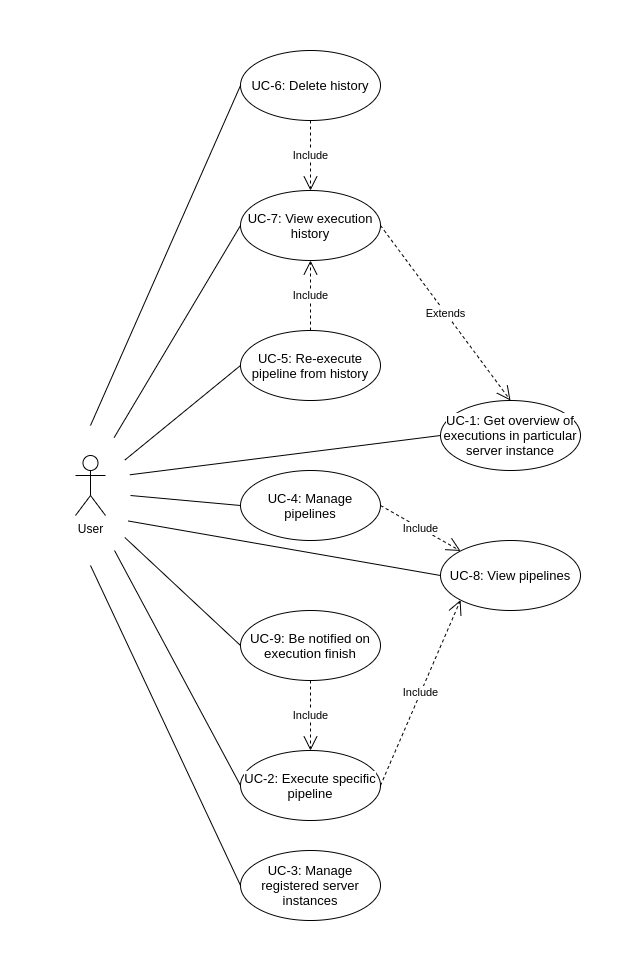
\includegraphics[width=0.9\textwidth]{pics/bc-uc.png}
	\caption[Use cases]{Diagram consisting of use cases}\label{fig:uc}
\end{figure}

%For better perspective, here is a diagram of all these use cases: \ref{fig:uc}

\subsection{Scenarios}
In this section, scenarios for users will be created.

\subsubsection*{SC-1.1: Get overview of executions in particular server instance}
User opens execution history screen and selects what server instance executions he wants to see.
\subsubsection*{SC-2.1: Execute specific pipeline}
User opens pipeline list screen. He then finds the desired pipeline and execute it. Optional: After opening the pipeline screen, user can filter pipelines by the server instance.
\subsubsection*{SC-3.1: Change IP address or name of registered server instance}
User opens settings screen, selects the desired server instance for edit. He then changes the IP address and saves changes.
\subsubsection*{SC-3.2: Register server instance}
User opens settings screen, tells the application he wants to register new server instance and proceeds to enter server instance info and saves it.
\subsubsection*{SC-3.3: Delete registered server instance}
User opens settings screen, views registered server instances and tells the application what server instance he wants to delete. It will be possible to undo the action.
\subsubsection*{SC-4.1: Create pipeline}
User opens pipeline list screen. Then he tells the application he wants to create a new pipeline. He chooses a server instance to which the pipeline will be saved and the screen for editing pipeline will be launched and the user can design a new pipeline here. When he is finished, he will save the pipeline.
\subsubsection*{SC-4.2: Edit pipeline}
User opens pipeline list screen. He then finds the desired pipeline and tells the application he wants to edit it. The screen for editing pipeline will be launched with the selected pipeline loaded so the user can make and save changes here. Optional: After opening the pipeline screen, user can filter pipelines by the server instance.
\subsubsection*{SC-4.3: Delete pipeline}
User opens pipeline list screen. He then finds the desired pipeline and tells the application he wants to delete it. It will be possible to undo the action. Optional: After opening the pipeline screen, user can filter pipelines by the server instance.
\subsubsection*{SC-5.1: Re-execute pipeline from history}
User opens execution history screen. He finds a pipeline and realize he wants to execute it now, so he tells that to the application. Optional: After opening the execution history screen, he can selects what server instance executions he wants to see.
\subsubsection*{SC-6.1: Delete history}
User opens execution history screen. He finds a record and realize he for some reason doesn't want this record in history anymore, so he tells that to the application. Optional: After opening the execution history screen, he can selects what server instance executions he wants to see.
\subsubsection*{SC-9.1: Be notified}
User executes specific pipeline, just like in SC-2.1. Application will notify user about the execution completion. This will happen only if it is allowed in settings.

\section{Specification}
The goal of this section is to produce a structured document consisting of functional requirements.

\subsection*{F-1.0: Settings screen}
Application must have a separate screen for settings. It can be seen in scenarios SC-3.1, SC-3.2, SC-3.3.
\subsection*{F-2.1: View server instance}
List of server instances will be visible from settings screen. It can be seen in scenarios SC-3.1, SC-3.3.
\subsection*{F-2.2: Add server instance}
User must be able to add server instance. It can be seen in scenarios SC-3.2.
\subsection*{F-2.3: Edit server instance}
User must be able to edit already added server instance. It can be seen in scenarios SC-3.1.
\subsection*{F-2.4: Delete server instance}
User must be able to delete already added server instance. It will be possible to undo the action. It can be seen in scenarios SC-3.3.
\subsection*{F-2.5: Deactivate server instance}
User can deactivate server instance in settings instead of deleting it, so it is possible to activate it again later easily. App will not communicate with deactivated server instances.
\subsection*{F-2.6: Ping server}
\label{subsec:ping}
User can test if the server address is correct
\subsection*{F-2.7: Load server instance info from qr code}
User can load server instance URL from qr code
\subsection*{F-3.1: Notification after finish}
\label{subsec:notifications}
Application shell create notification on pipeline finish. It can be seen in scenarios SC-9.1.
\subsection*{F-3.2: Notifications in settings}
There will be switch in settings to toggle notifications. It can be seen in scenarios SC-9.1.
\subsection*{F-4.0: Pipeline list screen}
Application must have a separate screen for working with pipelines. Which pipelines will be visible there depends on F-4.7. It can be seen in scenarios SC-2.1, SC-4.1, SC-4.2, SC-4.3.
\subsection*{F-4.1: View pipelines}
List of pipelines will be visible from pipeline list screen. Which pipelines will be visible depends on F-4.7. It can be seen in scenarios SC-2.1, SC-4.2, SC-4.3.
\subsection*{F-4.2: Edit pipeline screen}
\label{subsec:editpipelinescreen}
Application must have a screen for editing pipelines. It can be seen in scenarios SC-4.1, SC-4.2.
\subsection*{F-4.3: Create pipelines}
User must be able to start an empty edit pipeline screen (F-4.2) from the pipeline list screen (F-4.0). It can be seen in scenarios SC-4.1.
\subsection*{F-4.4: Edit existing pipelines}
User must be able to edit selected pipeline by starting the edit pipeline screen (F-4.2) with the selected pipeline loaded. It can be seen in scenarios SC-4.2.
\subsection*{F-4.5: Delete pipelines}
User must be able to delete a pipeline of his choice. It can be seen in scenarios SC-4.3.
\subsection*{F-4.6: Execute pipeline}
User must be able to execute selected pipeline. It can be seen in scenarios SC-2.1.
\subsection*{F-4.7: Source for visible pipelines}
User must be able to choose, if he wants to see pipelines from all instances, or just a specific one. It can be seen in scenarios SC-2.1, SC-4.2, SC-4.3.
\subsection*{F-5.0: Execution history screen}
Application must have a separate screen for execution history. History of which server instance will be visible depends on F-5.4 It can be seen in scenarios SC-1.1, SC-5.1, SC-6.1.
\subsection*{F-5.1: View execution history}
List of executions will be visible from the execution history screen. History of which server instance will be visible depends on F-5.4 It can be seen in scenarios SC-1.1, SC-5.1, SC-6.1.
\subsection*{F-5.2: Delete items from history}
User must be able to delete specific item from execution history. It will be possible to undo the action. It can be seen in scenarios SC-6.1.
\subsection*{F-5.3: Re-execute pipelines from history}
There must be an option to re-execute pipeline from the execution history screen. This action will also make a new record in execution history. It can be seen in scenarios SC-5.1.
\subsection*{F-5.4: Source of visible history}
User must be able to choose, if he wants to see history of all instances, or just a specific one. It can be seen in scenarios SC-1.1, SC-5.1, SC-6.1.
\subsection*{F-6.1: Night mode}
User can have an option in settings to use light or dark theme, or use system default theme (Android 10 and newer).

%
%\chapter{Existing solutions}
%If there already exists a perfect solution which suits our requirements, it doesn't make sense to create it one more time.
\todo[inline]{Jazyk! Nepoužívejte zkratky (doesn't). A opět, napište, co v sekci bude, ne coby kdyby. Tedy přehled existujících řešení. Nepište, že pokud existuje, nemá cenu ho dělat znovu. }

\todo[inline]{Takto bude sekce působit (a se stylystického pohledu bude hodnocena) jako nevyvážená. Je příliš krátká.}
\todo[inline]{Navíc používáte osamocené podnadpisy (tj. že zavádíte další úroveň nadpisu, např. 2.1.1, a přitom je v té úrovni jen jeden (není žádný 2.1.2). Tedy buďto úroveň nezavádějte, nebo dodejte další obsah pod další nadpis.}

\section{Description of existing solutions}
Here is a brief description of solutions that already exist.

\subsection{Responsive web app}
The web front-end can be used by any device possessing a web browser.
\todo[inline]{use formal language}
%It \todo[inline]{what is "it"?} works on any device \todo[inline]{so, a typewriter?}, not just android devices.
%\todo[inline]{this reads like a concept of a blog post, not like a formal message.}
Users don't have to download any application, which also means they don't have to update it.
The responsive web app only works with one server instance.
On an Android device, it responds slower to screen rotation and animations often lag.
% Even if you don't want to execute anything, just view history or list pipelines, you have to be online.
Even if users don't want to execute anything, just view history or list pipelines, they have to be online.
It is also browser dependent.

\section{Summary of existing solutions}
In this section, existing solutions are being compared with each other (see \autoref{tab:existingSolutions}), resulting in a decision if there is a need to create new application.
\todo[inline]{each heading needs to be followed by a text and not another heading. What is the contents of this section, briefly?}

\begin{table}[ht]\centering
\caption[Existing solutions]{Features of existing solutions}\label{tab:existingSolutions}
\begin{tabular}{l|l|l}
\hline
\textbf{Feature} & \textbf{Android App} & \textbf{Web App} \\ \hline
Can work with multiple server instances & + & - \\ \hline
Works on any device & - & + \\ \hline
Doesn't need to be downloaded & - & + \\ \hline
Smooth UI & + & - \\ \hline
Can view stuff while offline & + & - \\ \hline
\end{tabular}
\end{table}

The comparison indicates that the web application is missing at least one critical feature, that is not being able to work with multiple server instances, thus there is a need for the creation of new application.
%
%\chapter{Design}
%The appearance of the UI will be described in this chapter.

\section{Design language and UI framework}
Because the application should look decent, some UI guidelines have to be chosen and followed.
These guidelines cover information about colors, shapes and individual components, including their layout.
A set of these guidelines is called design language.
Following design languages are suitable for the Android platform due to the existence of frameworks for this platform, containing themes and components of those languages.

Bootstrap \cite{bootstrap} is a framework for designing web pages, but there also exists a third party library \cite{androidbootstrap} for the Android platform.
Both Microsoft Fluent Design System \cite{fluentui} and Material Design \cite{materialandroid} have their own official libraries available from their representative web pages.

The Bootstrap Android library has not been updated since December 2016 and considering that UI design is always changing and evolving, this library is out of question.
Both Microsoft Fluent Design System and Material Design are being kept up-to-date and are backed by big international companies, which should ensure their stability.
Because our application will be available on the Android platform, which is Google's domain and most Android phones come with several Google applications pre-installed, Android users are already used to Material Design.

That is why Material Design will be used by our application.

\section{Main screens}
Based on the analysis of the user requirements in \autoref{chap:requirementsengineering}, three screens which cover the functionality of displaying execution history, pipeline list and settings have to be designed.

\section{Main navigation}
On the Android platform, there are multiple navigation designs and they will be described in this section.

\subsection{Navigation drawer}
The hamburger icon at the top left and sliding menu from left to right is what the navigation drawer looks like.
This navigation is suitable for five or more top level screens, or some sort of hierarchical menu \cite{navigationdrawer}.

\subsection{Tabs}
Slidable tabs on top of the screen.
% Recommendation for this type of navigation is having at least two screens.\cite{materialandroid}
Users can click on tab names or just slide left or right in order to navigate between the screens.

\subsection{Bottom navigation}
Bottom navigation consists of icons, usually with text, located at the bottom of the screen.

\section{Conclusion about the main navigation}
The navigation drawer will not be used, because our application does not require five or more main screens nor a hierarchical menu.
Also, with the increasing sizes of mobile phones and most people being right-handed, it is hard to reach the hamburger menu with the right thumb.
There will be lists of items displayed on each of the three main screens.
Those items will be swipeable and having swipeable items on top of swipeable navigation would cause confusion.
Material Design states that the recommended number of links in the bottom navigation is three to five \cite{bottomnavigation}.
The bottom navigation satisfies our needs and will be used for the main navigation.
The three main screens, containing the bottom navigation, can be seen in \autoref{fig:xdHistory}, \autoref{fig:xdPipelines} and \autoref{fig:xdSettings}.

\begin{figure}\centering
    \begin{minipage}[b]{0.32\textwidth}
    	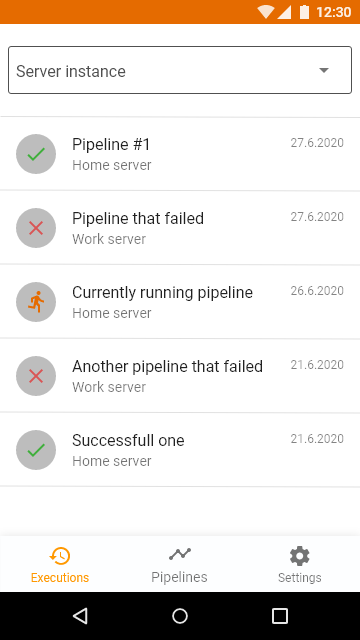
\includegraphics[width=\textwidth]{pics/xd/Bottom Navigation - executions.png}
    	\caption[History]{History screen design}\label{fig:xdHistory}
    \end{minipage}
    \begin{minipage}[b]{0.32\textwidth}
    	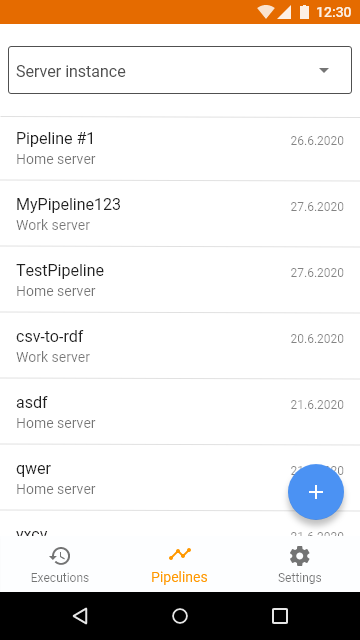
\includegraphics[width=\textwidth]{pics/xd/Bottom Navigation - pipelines.png}
    	\caption[Pipelines]{Pipelines screen design}\label{fig:xdPipelines}
    \end{minipage}
    \begin{minipage}[b]{0.32\textwidth}
    	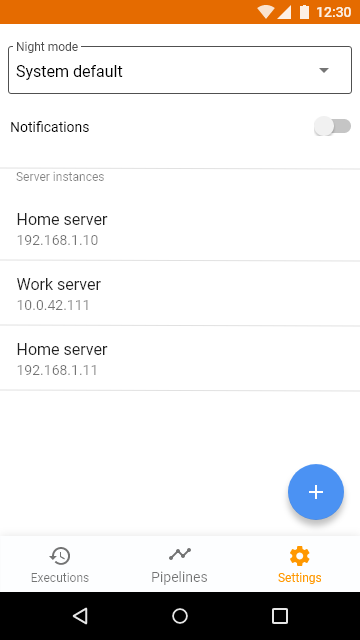
\includegraphics[width=\textwidth]{pics/xd/Bottom Navigation - settings.png}
    	\caption[Settings]{Settings screen design}\label{fig:xdSettings}
    \end{minipage}
\end{figure}

\section{Lists}
Each of the three main screens will display some sort of list.
For the execution screen it is a list of executions, for the pipeline screen it is a list of pipelines and for the settings screen it is a list of server instances.

All of those lists will have one thing in common and that being the swipe gesture.
When users swipe an item to the left or to the right, the item will be deleted.
This can be seen in \autoref{fig:xdDeletePipeline}.
Users will have the ability to undo this operation for a short period of time.
The undo option can be seen in \autoref{fig:xdUndo}.

Tapping on an item from the pipeline screen will open the edit pipeline screen.
Long click on item from execution screen or from pipeline screen will launch the pipeline.

\begin{figure}\centering
    \begin{minipage}[b]{0.32\textwidth}
    	\includegraphics[width=\textwidth]{pics/xd/Bottom Navigation - pipelines – 1.png}
    	\caption[Deleting pipeline]{Deleting pipeline design}\label{fig:xdDeletePipeline}
    \end{minipage}
    \begin{minipage}[b]{0.32\textwidth}
    	\includegraphics[width=\textwidth]{pics/xd/Bottom Navigation - pipelines – 2.png}
    	\caption[Undo option]{Undo option design}\label{fig:xdUndo}
    \end{minipage}
\end{figure}

\section{Edit server instance screen}
While registering a new server instance or editing an already registered one, the application needs the address for communication and some name for labeling and better organising.
Users will be able to add a description of the instance, so that there is no pressure to store every information about the instance in the server name.
There could also be an option to ping the server (F-2.6, \autoref{subsec:ping}) to verify the address and a way to cancel the registration/edit.
Because of this, another screen, just for registering/editing server instances, will be added and can be seen in \autoref{fig:xdEditServerInstance}.

\begin{figure}\centering
    \begin{minipage}[b]{0.32\textwidth}
    	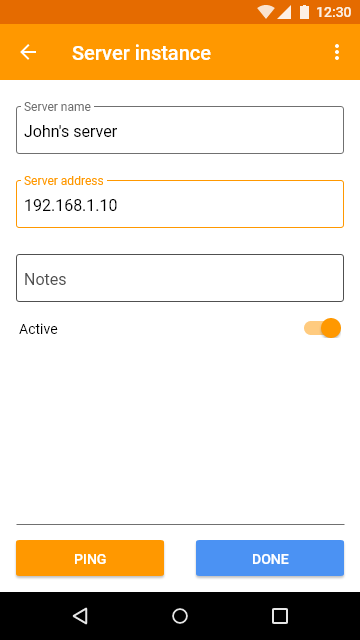
\includegraphics[width=\textwidth]{pics/xd/Edit server instance.png}
    	\caption[Edit server instance]{Edit server instance screen design}\label{fig:xdEditServerInstance}
    \end{minipage}
    \begin{minipage}[b]{0.32\textwidth}
    	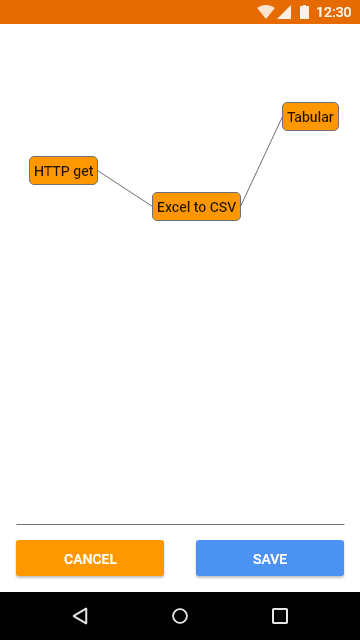
\includegraphics[width=\textwidth]{pics/xd/Pipeline editor.png}
    	\caption[Edit pipeline screen]{Edit pipeline screen design}\label{fig:xdPipelineEditor}
    \end{minipage}
\end{figure}

\section{Edit pipeline screen}
According to the F-4.3 requirement, described in \autoref{subsec:editpipelinescreen}, there has to be a screen for editing pipelines.
This screen will be displaying pipeline components and drawing links between them.
The preliminary design of this screen can be seen in \autoref{fig:xdPipelineEditor}

% \begin{figure}\centering
%     \begin{minipage}[b]{0.32\textwidth}
%     	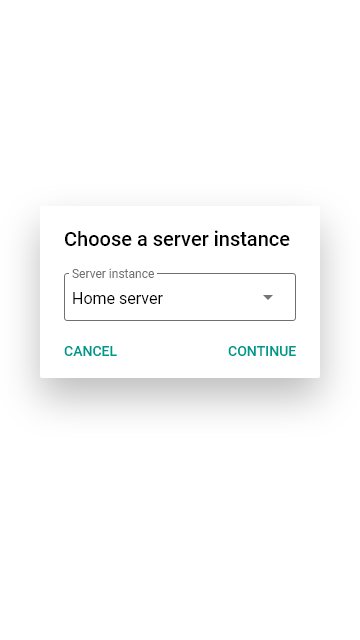
\includegraphics[width=\textwidth]{pics/xd/Create new pipeline.png}
%     	\caption[Create new pipeline dialog]{Create new pipeline dialog design}\label{fig:xdCreateNewPipelineDialog}
%     \end{minipage}
%     \begin{minipage}[b]{0.32\textwidth}
%     	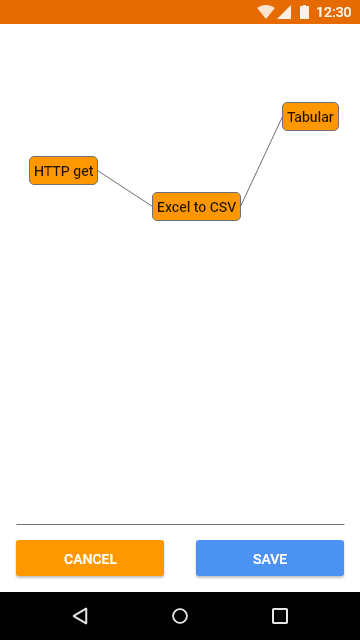
\includegraphics[width=\textwidth]{pics/xd/Pipeline editor.png}
%     	\caption[Edit pipeline screen]{Edit pipeline screen design}\label{fig:xdPipelineEditor}
%     \end{minipage}
% \end{figure}

\section{Edit component screen}
This screen has to be created, because each pipeline's component has its own settings.
In \autoref{fig:xdEditComponent1} and \autoref{fig:xdEditComponent2} is the preliminary design of this screen.

\begin{figure}\centering
    \begin{minipage}[b]{0.32\textwidth}
    	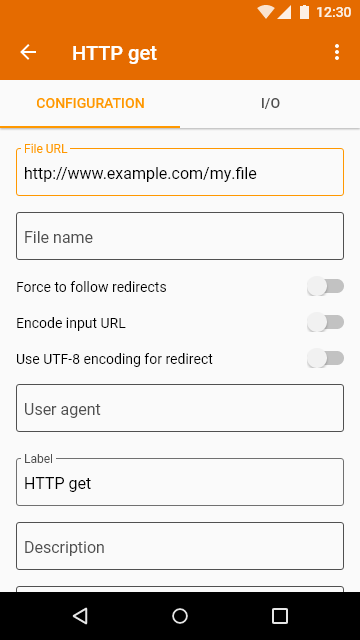
\includegraphics[width=\textwidth]{pics/xd/Edit component - configuration.png}
    	\caption[Edit component screen 1]{Edit component screen 1 design}\label{fig:xdEditComponent1}
    \end{minipage}
    \begin{minipage}[b]{0.32\textwidth}
    	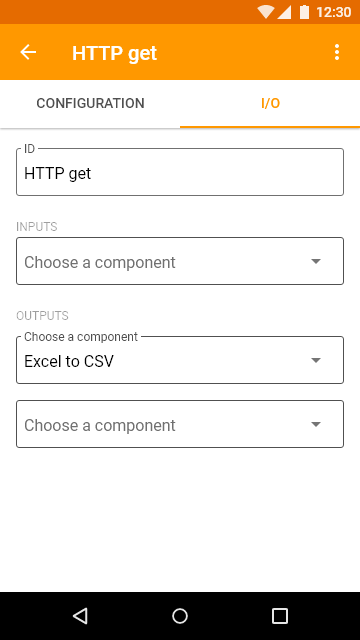
\includegraphics[width=\textwidth]{pics/xd/Edit component - io.png}
    	\caption[Edit component screen 2]{Edit component screen 2 design}\label{fig:xdEditComponent2}
    \end{minipage}
\end{figure}

\section{Notifications}
According to the F-3.1 requirement, described in \autoref{subsec:notifications}, notifications need to be implemented.
The preview of notifications can be seen in \autoref{fig:xdNotifications}.

\begin{figure}\centering
    \begin{minipage}[b]{0.7\textwidth}
    	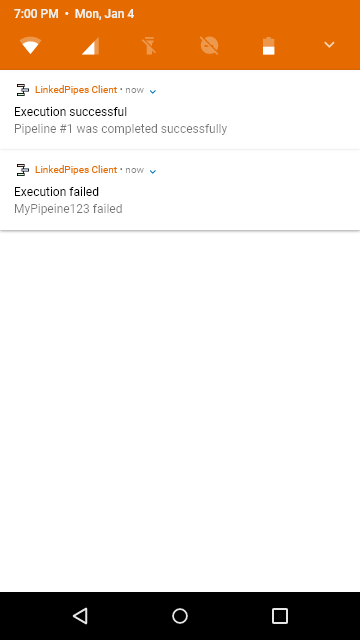
\includegraphics[width=\textwidth]{pics/xd/Notifications.png}
    	\caption[Notifications]{Notification design}\label{fig:xdNotifications}
    \end{minipage}
\end{figure}
%% https://www.youtube.com/watch?v=ugpC98LcNqA
% https://www.youtube.com/watch?v=QrbhPcbZv0I

\section{Software architecture patterns}
Every non trivial software project should follow some architecture design.
But why? You want your project to be always maintainable and expandable as much easily as possible.
You want to modularize it, so that you can just take one part and exchange it without the need of rewriting the whole project.
And for this reason, there are architecture patterns.
I will describe three of them and explain my conclusion.

All of these three patterns have one thing in common.
They structure code into three main layers.
The names of those layers are present in these pattern's names.

\subsection{MVC}

\begin{figure}\centering
	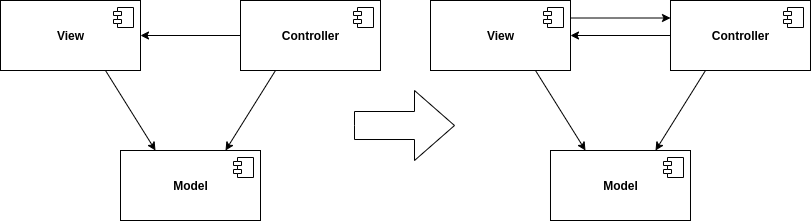
\includegraphics[width=1\textwidth]{pics/patterns/bc-mvc2.png}
	\caption[MVC]{Model View Controller}\label{fig:mvc}
\end{figure}

\textbf{Model View Controller}.
View is responsible for displaying data, controller is responsible for getting the user input and model for storing data.
The controller takes user input, it updates the model and then tells the view to update itself.

Now we know, that if we choose this, it will be implemented in android.
How does one do this? In the android world, the part of application responsible for displaying things is also responsible for dealing with user input.
So you tweak the pattern so the view gets the user input, it sends it to the controller, the controller updates the model, then tells the view to update itself, based on the data from model.

So both view and controller know the model, the view knows controller and controller knows view.
That's pretty bad, you don't want this.
That's high consistency and that is a thing you want to avoid, especially in the android world, where forgetting to remove a link can and will cause memory leaks.

And what if you want to somehow transform the data for presentation?
What part should do this presentation transformation, also known as UI logic?
You don't want to push this to the view, because you want the UI logic also to be easily testable and you want to separate it from the appearance of the view.
Controller can not posses it neither, because it doesn't supply any data to the view. So should you put it in the model? Absolutely not!
Why should a part of the application, responsible for data storing, know how to display stuff?

\subsection{MVP}

\begin{figure}\centering
	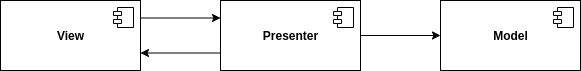
\includegraphics[width=0.7\textwidth]{pics/patterns/bc-mvp.png}
	\caption[MVP]{Model View Presenter}\label{fig:mvp}
\end{figure}

Imagine the MVC and the UI logic problem.
Now what if the view doesn't communicate with the model, but only with controller and the controller was also responsible for taking data from the model and supplying them to the view.
Then you would be able to put UI logic to this new controller. Now we will call it presenter, instead of new controller.
And that's what \textbf{Model View Presenter} is.

But that means the presenter still holds a link to the view. You still need to write some repetitive code because of this.
Second, why would the presenter should know, what parts of the view should be updated after the data changes?

\subsection{MVVM}

\begin{figure}\centering
	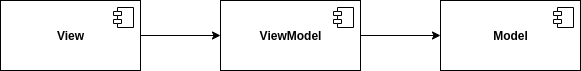
\includegraphics[width=0.7\textwidth]{pics/patterns/bc-mvvm.png}
	\caption[MVVM]{Model View ViewModel}\label{fig:mvvm}
\end{figure}

\textbf{Model View Viewmodel}.
We will borrow the MVP and tweak it a little. Currently the presenter knows the view and is executing it's methods when it needs to be updated.
Let's rename presenter to viewmodel. It no longer knows it's view.
Instead it provides some kind of stream and the view can observe the stream, so it can do whatever whenever it omits any data.

So the view knows the viewmodel, can call it's methods on user input and observe it's data streams.
The viewmodel knows model, observes it's data streams and omits them to the view.
The view knows the viewmodel, the viewmodel knows the model and the model don't know any of them.

\subsection{And the winner is ...}
Our choice is MVVM. Not only it looks like the tip of the evolution, but Google even made some libraries to support it.

\section{Main layers and libraries}
We will go over the three main layers of the MVVM, add a fourth at the end and describe some libraries that will be used inside of them.

\subsection{View}
As I said before, the view is the layer responsible for displaying data. It's what I call a screen in functional requirements.
The way it's implemented is through a combination of standard kotlin code and xml.
The xml is like a skeleton and kotlin is like life. In xml, you specify the look and in kotlin, you can specify what data it should display, how to update itself and what to do with user input.

For that, you have to somehow link or bind these two things (xml and kotlin) together.
We will be using a library called Data Binding. It's better than nothing and compared to other solutions, like kotlin's synthetics, Data Binding offers more features and I personally think it looks clearer.

\subsection{Viewmodel}
Google has made some architecture components and one of them is exactly for viewmodel.
It will be shame not to use it.

\subsection{Repository}
Repository will represent the model.
It's a place responsible for maintaining data.
Does the application need to download them, or load from cache?
Do you need to get anything out of the application or get anything in it?
You will ask the repository, also known as the one and the only source of truth.

\subsection{DAO and network IO}
This will be the fourth layer.
Every android app can run it's own SQLite database.
Data Access Objects will be used to access data in in this database.
There is a nice library for that called Room and we will be using it.
Network IO layer will be responsible for communication with server instance API.
We will be using Retrofit library for those API requests.
Repository will be using both of those in order to maintain and organise data.

\subsection{LiveData}
LiveData is a library.
It will be used in each layer.
Previously I talked about observing some kind of stream.
For this, you need some kind of observable variables and that's what LiveData is.
It enables you to set some action to happen when the data changes.
LiveData is not just some ordinary stream, it only streams, when there is some observer living.
It may sound silly, but for example, you don't need to update certain screen, when that screen is not visible.

\section{Conclusion}

\begin{figure}\centering
	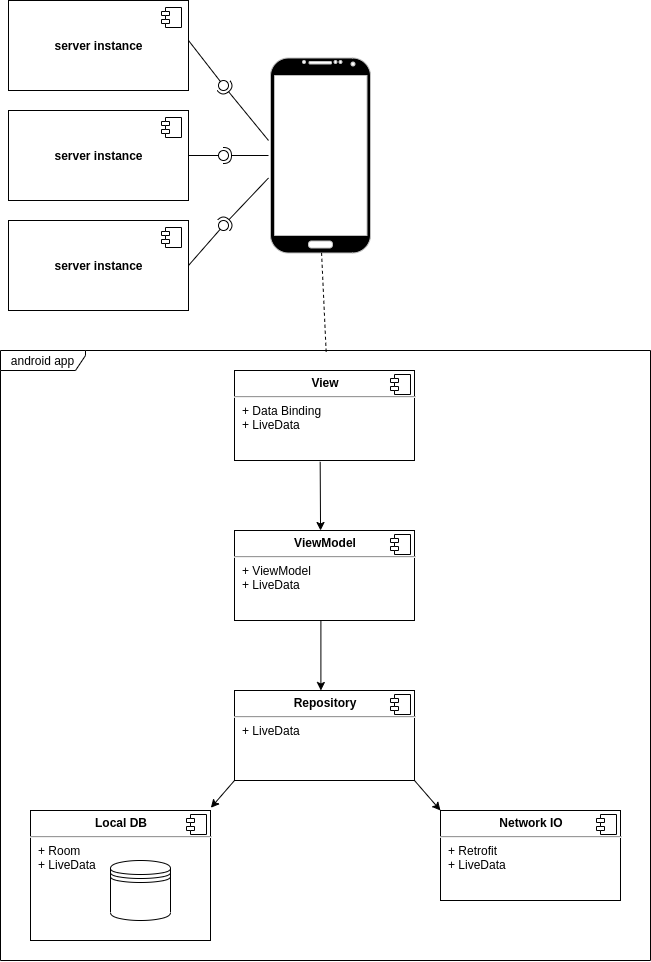
\includegraphics[width=1\textwidth]{pics/bc-architecture.png}
	\caption[Architecture]{Diagram consisting of MVVM and server instances}\label{fig:architecture}
\end{figure}

For better perspective, here is a summarizing diagram: \ref{fig:architecture}

The android device will communicate directly with multiple server instances. Network IO layer will be responsible for this communication. Repository will cache it using the Local DB layer and hand out data to the viewmodel. Viewmodel can do any UI logic that's needed and pass it to the view. All handing out or passing from any bottom layer to the one on top will be done through the observation of LiveData.
%
%%\chapter{Realization}
%\chapter{Implementation}
%//TODO
%
%\chapter{Deployment}
%//TODO

\chapter{Work goal}
The goal of this thesis is to pitch an Android client for the \etl{} system as an alternative to opening a web page in a mobile browser.

In order to do that, following steps must be fulfilled.

\begin{itemize}
    \item A list of requirements for the application will be put together in the analysis chapter.
    \item Existence of no current solution will be verified in the existing solutions chapter.
    \item Application will be designed, including appearance and code layering, in the design chapters.
    \item Result of the implementation chapter will be the application.
    \item Documentation will be created after the application is created and described in the documentation chapter.
    \item Application tests will be described in the test chapter.
\end{itemize}

%\input{chapters/testing}
%% % % % % % % % % % % % % % % % % % % % % % % % % % % % 
% Tuto kapitolu z výsledné práce ODSTRAŇTE.
% % % % % % % % % % % % % % % % % % % % % % % % % % % 

\chapter{Návod k~použití této šablony}

Tento dokument slouží jako základ pro napsání závěrečné práce na Fakultě informačních technologií ČVUT v~Praze.

\section{Výběr základu}

Vyberte si šablonu podle druhu práce (bakalářská, diplomová), jazyka (čeština, angličtina) a kódování (ASCII, \mbox{UTF-8}, \mbox{ISO-8859-2} neboli latin2 a nebo \mbox{Windows-1250}). 

V~české variantě naleznete šablony v~souborech pojmenovaných ve formátu práce\_kódování.tex. Typ může být:
\begin{description}
	\item[BP] bakalářská práce,
	\item[DP] diplomová (magisterská) práce.
\end{description}
Kódování, ve kterém chcete psát, může být:
\begin{description}
	\item[UTF-8] kódování Unicode,
	\item[ISO-8859-2] latin2,
	\item[Windows-1250] znaková sada 1250 Windows.
\end{description}
V~případě nejistoty ohledně kódování doporučujeme následující postup:
\begin{enumerate}
	\item Otevřete šablony pro kódování UTF-8 v~editoru prostého textu, který chcete pro psaní práce použít -- pokud můžete texty s~diakritikou normálně přečíst, použijte tuto šablonu.
	\item V~opačném případě postupujte dále podle toho, jaký operační systém používáte:
	\begin{itemize}
		\item v~případě Windows použijte šablonu pro kódování \mbox{Windows-1250},
		\item jinak zkuste použít šablonu pro kódování \mbox{ISO-8859-2}.
	\end{itemize}
\end{enumerate}


V~anglické variantě jsou šablony pojmenované podle typu práce, možnosti jsou:
\begin{description}
	\item[bachelors] bakalářská práce,
	\item[masters] diplomová (magisterská) práce.
\end{description}

\section{Použití šablony}

Šablona je určena pro zpracování systémem \LaTeXe{}. Text je možné psát v~textovém editoru jako prostý text, lze však také využít specializovaný editor pro \LaTeX{}, např. Kile.

Pro získání tisknutelného výstupu z~takto vytvořeného souboru použijte příkaz \verb|pdflatex|, kterému předáte cestu k~souboru jako parametr. Vhodný editor pro \LaTeX{} toto udělá za Vás. \verb|pdfcslatex| ani \verb|cslatex| \emph{nebudou} s~těmito šablonami fungovat.

Více informací o~použití systému \LaTeX{} najdete např. v~\cite{wikilatex}.

\subsection{Typografie}

Při psaní dodržujte typografické konvence zvoleného jazyka. České \uv{uvozovky} zapisujte použitím příkazu \verb|\uv|, kterému v~parametru předáte text, jenž má být v~uvozovkách. Anglické otevírací uvozovky se v~\LaTeX{}u zadávají jako dva zpětné apostrofy, uzavírací uvozovky jako dva apostrofy. Často chybně uváděný symbol "{} (palce) nemá s~uvozovkami nic společného.

Dále je třeba zabránit zalomení řádky mezi některými slovy, v~češtině např. za jednopísmennými předložkami a spojkami (vyjma \uv{a}). To docílíte vložením pružné nezalomitelné mezery -- znakem \texttt{\textasciitilde}. V~tomto případě to není třeba dělat ručně, lze použít program \verb|vlna|.

Více o~typografii viz \cite{kobltypo}.

\subsection{Obrázky}

Pro umožnění vkládání obrázků je vhodné použít balíček \verb|graphicx|, samotné vložení se provede příkazem \verb|\includegraphics|. Takto je možné vkládat obrázky ve formátu PDF, PNG a JPEG jestliže používáte pdf\LaTeX{} nebo ve formátu EPS jestliže používáte \LaTeX{}. Doporučujeme preferovat vektorové obrázky před rastrovými (vyjma fotografií).

\subsubsection{Získání vhodného formátu}

Pro získání vektorových formátů PDF nebo EPS z~jiných lze použít některý z~vektorových grafických editorů. Pro převod rastrového obrázku na vektorový lze použít rasterizaci, kterou mnohé editory zvládají (např. Inkscape). Pro konverze lze použít též nástroje pro dávkové zpracování běžně dodávané s~\LaTeX{}em, např. \verb|epstopdf|.

\subsubsection{Plovoucí prostředí}

Příkazem \verb|\includegraphics| lze obrázky vkládat přímo, doporučujeme však použít plovoucí prostředí, konkrétně \verb|figure|. Například obrázek \ref{fig:float} byl vložen tímto způsobem. Vůbec přitom nevadí, když je obrázek umístěn jinde, než bylo původně zamýšleno -- je tomu tak hlavně kvůli dodržení typografických konvencí. Namísto vynucování konkrétní pozice obrázku doporučujeme používat odkazování z~textu (dvojice příkazů \verb|\label| a \verb|\ref|).

\begin{figure}\centering
	
\includegraphics[width=0.5\textwidth, angle=30]{cvut-logo-bw}
	\caption[Příklad obrázku]{Ukázkový obrázek v~plovoucím prostředí}\label{fig:float}
\end{figure}

\subsubsection{Verze obrázků}

% Gnuplot BW i barevně
Může se hodit mít více verzí stejného obrázku, např. pro barevný či černobílý tisk a nebo pro prezentaci. S~pomocí některých nástrojů na generování grafiky je to snadné.

Máte-li například graf vytvořený v programu Gnuplot, můžete jeho černobílou variantu (viz obr. \ref{fig:gnuplot-bw}) vytvořit parametrem \verb|monochrome dashed| příkazu \verb|set term|. Barevnou variantu (viz obr. \ref{fig:gnuplot-col}) vhodnou na prezentace lze vytvořit parametrem \verb|colour solid|.


\subsection{Tabulky}

Tabulky lze zadávat různě, např. v~prostředí \verb|tabular|, avšak pro jejich vkládání platí to samé, co pro obrázky -- použijte plovoucí prostředí, v~tomto případě \verb|table|. Například tabulka \ref{tab:matematika} byla vložena tímto způsobem.

\begin{table}\centering
	\caption[Příklad tabulky]{Zadávání matematiky}\label{tab:matematika}
	\begin{tabular}{|l|l|c|c|}\hline
		Typ		& Prostředí		& \LaTeX{}ovská zkratka	& \TeX{}ovská zkratka	\tabularnewline \hline \hline
		Text		& \verb|math|		& \verb|\(...\)|	& \verb|$...$|		\tabularnewline \hline
		Displayed	& \verb|displaymath|	& \verb|\[...\]|	& \verb|$$...$$|	\tabularnewline \hline
	\end{tabular}
\end{table}

% % % % % % % % % % % % % % % % % % % % % % % % % % % 

\chapter{Requirements engineering}
%Requirements engineering is a process to determine things, the desired system will consist of. This process itself consists of three stages.
Things \todo[inline]{what things? - a není to pravda. To, z čeho se systém skládá, je desgin. Analýza řeši, co bude systém dělat.} the desired system will consist of will be determined in this chapter by going through following three stages. \todo[inline]{co jsou ty stages? to, že to jsou pak nadpisy podkapitol nestačí.}

\section{Elicitation}
\todo[inline]{Nadpis: Elicitaion čeho?}
Raw information \todo[inline]{myslíte user requirements?} about a desired application will be gathered here.
These two sentences were gathered:
\begin{itemize}
    \item It will be an android-based mobile application serving as an alternative client to the current \etl{} front-end.
    \item The application will provide pipeline and execution management and notification capabilities for multiple \etl{} instances.
\end{itemize}

\section{Analysis}
Analysis phase is about making sense from elicitation.
It's a systematic approach to elicitation.

\todo[inline]{Need to restructure: First, you get requirements. Then you analyze them and create use cases. Each use case represents a goal the user wants to achieve using the app.  Each use case has a user scenario describing approximately what steps need to be taken to achieve the goal. Since here, you do not have the design ready, it does not have to be click-by-click. Each use case should cover some requirements, and you should specify which.}

\subsection{Use cases}
One good method of achieving this is by describing some use cases.
Each use case is something that users expect from the system.
Scenarios will be created for the non trivial ones.
Scenario is an array of tasks user should do in order to go through the use case.

\subsubsection*{UC-1: Get overview of executions in particular server instance}
Enables user to see what pipelines were executed in chronological order from specific server instance.
\subsubsection*{UC-2: Execute specific pipeline}
Enables user to execute pipeline of his choice from specific server instance.
\subsubsection*{UC-3: Manage registered server instances}
Enables user to register server instance in the application. Application will check, if IP is already registered or if name of the new server instance is already in use, in order to warn user about duplication or name collision that could cause chaos. It also enables user to change IP address of already registered server instance due to type error or network changes. User can also remove registered server instance.
\subsubsection*{UC-4: Manage pipelines}
Enables user to manage pipelines in desired server instance.
\subsubsection*{UC-5: Re-execute pipeline from history}
Enables user to quickly execute pipeline he stumbles upon while viewing history.
\subsubsection*{UC-6: Delete history}
Enables user to delete items from history.
\subsubsection*{UC-7: View execution history}
Enables user to view execution history of all the instances at the same time.
\subsubsection*{UC-8: View pipelines}
Enables user to view pipelines from all the server instances.
\subsubsection*{UC-9: Be notified on execution finish}
User has the option to be notified about execution completion.

%\subsubsection*{Diagram}
\begin{figure}\centering
	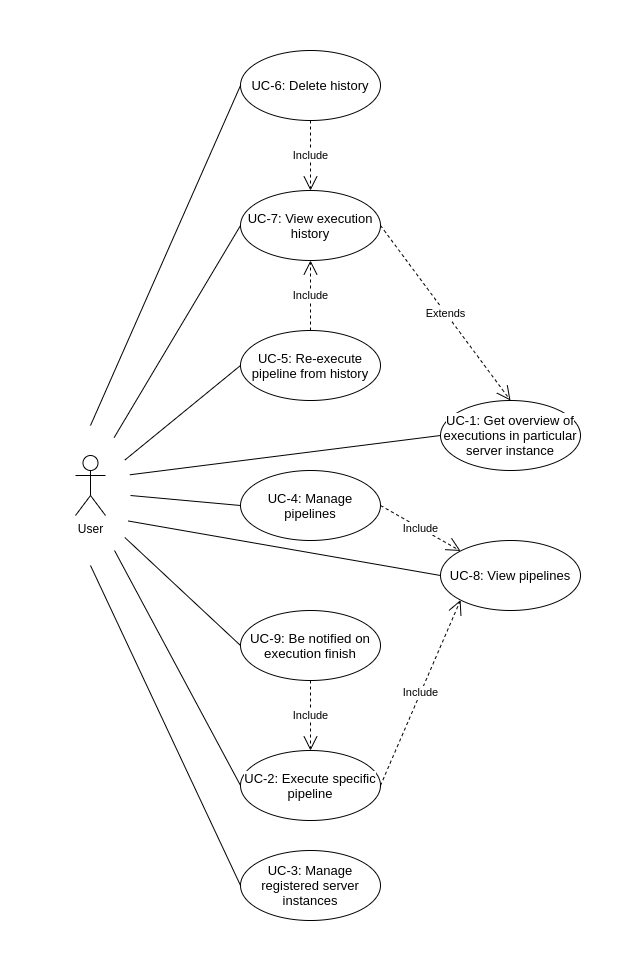
\includegraphics[width=0.9\textwidth]{pics/bc-uc.png}
	\caption[Use cases]{Diagram consisting of use cases}\label{fig:uc}
\end{figure}

%For better perspective, here is a diagram of all these use cases: \ref{fig:uc}

\subsection{Scenarios}
In this section, scenarios for users will be created.

\subsubsection*{SC-1.1: Get overview of executions in particular server instance}
User opens execution history screen and selects what server instance executions he wants to see.
\subsubsection*{SC-2.1: Execute specific pipeline}
User opens pipeline list screen. He then finds the desired pipeline and execute it. Optional: After opening the pipeline screen, user can filter pipelines by the server instance.
\subsubsection*{SC-3.1: Change IP address or name of registered server instance}
User opens settings screen, selects the desired server instance for edit. He then changes the IP address and saves changes.
\subsubsection*{SC-3.2: Register server instance}
User opens settings screen, tells the application he wants to register new server instance and proceeds to enter server instance info and saves it.
\subsubsection*{SC-3.3: Delete registered server instance}
User opens settings screen, views registered server instances and tells the application what server instance he wants to delete. It will be possible to undo the action.
\subsubsection*{SC-4.1: Create pipeline}
User opens pipeline list screen. Then he tells the application he wants to create a new pipeline. He chooses a server instance to which the pipeline will be saved and the screen for editing pipeline will be launched and the user can design a new pipeline here. When he is finished, he will save the pipeline.
\subsubsection*{SC-4.2: Edit pipeline}
User opens pipeline list screen. He then finds the desired pipeline and tells the application he wants to edit it. The screen for editing pipeline will be launched with the selected pipeline loaded so the user can make and save changes here. Optional: After opening the pipeline screen, user can filter pipelines by the server instance.
\subsubsection*{SC-4.3: Delete pipeline}
User opens pipeline list screen. He then finds the desired pipeline and tells the application he wants to delete it. It will be possible to undo the action. Optional: After opening the pipeline screen, user can filter pipelines by the server instance.
\subsubsection*{SC-5.1: Re-execute pipeline from history}
User opens execution history screen. He finds a pipeline and realize he wants to execute it now, so he tells that to the application. Optional: After opening the execution history screen, he can selects what server instance executions he wants to see.
\subsubsection*{SC-6.1: Delete history}
User opens execution history screen. He finds a record and realize he for some reason doesn't want this record in history anymore, so he tells that to the application. Optional: After opening the execution history screen, he can selects what server instance executions he wants to see.
\subsubsection*{SC-9.1: Be notified}
User executes specific pipeline, just like in SC-2.1. Application will notify user about the execution completion. This will happen only if it is allowed in settings.

\section{Specification}
The goal of this section is to produce a structured document consisting of functional requirements.

\subsection*{F-1.0: Settings screen}
Application must have a separate screen for settings. It can be seen in scenarios SC-3.1, SC-3.2, SC-3.3.
\subsection*{F-2.1: View server instance}
List of server instances will be visible from settings screen. It can be seen in scenarios SC-3.1, SC-3.3.
\subsection*{F-2.2: Add server instance}
User must be able to add server instance. It can be seen in scenarios SC-3.2.
\subsection*{F-2.3: Edit server instance}
User must be able to edit already added server instance. It can be seen in scenarios SC-3.1.
\subsection*{F-2.4: Delete server instance}
User must be able to delete already added server instance. It will be possible to undo the action. It can be seen in scenarios SC-3.3.
\subsection*{F-2.5: Deactivate server instance}
User can deactivate server instance in settings instead of deleting it, so it is possible to activate it again later easily. App will not communicate with deactivated server instances.
\subsection*{F-2.6: Ping server}
\label{subsec:ping}
User can test if the server address is correct
\subsection*{F-2.7: Load server instance info from qr code}
User can load server instance URL from qr code
\subsection*{F-3.1: Notification after finish}
\label{subsec:notifications}
Application shell create notification on pipeline finish. It can be seen in scenarios SC-9.1.
\subsection*{F-3.2: Notifications in settings}
There will be switch in settings to toggle notifications. It can be seen in scenarios SC-9.1.
\subsection*{F-4.0: Pipeline list screen}
Application must have a separate screen for working with pipelines. Which pipelines will be visible there depends on F-4.7. It can be seen in scenarios SC-2.1, SC-4.1, SC-4.2, SC-4.3.
\subsection*{F-4.1: View pipelines}
List of pipelines will be visible from pipeline list screen. Which pipelines will be visible depends on F-4.7. It can be seen in scenarios SC-2.1, SC-4.2, SC-4.3.
\subsection*{F-4.2: Edit pipeline screen}
\label{subsec:editpipelinescreen}
Application must have a screen for editing pipelines. It can be seen in scenarios SC-4.1, SC-4.2.
\subsection*{F-4.3: Create pipelines}
User must be able to start an empty edit pipeline screen (F-4.2) from the pipeline list screen (F-4.0). It can be seen in scenarios SC-4.1.
\subsection*{F-4.4: Edit existing pipelines}
User must be able to edit selected pipeline by starting the edit pipeline screen (F-4.2) with the selected pipeline loaded. It can be seen in scenarios SC-4.2.
\subsection*{F-4.5: Delete pipelines}
User must be able to delete a pipeline of his choice. It can be seen in scenarios SC-4.3.
\subsection*{F-4.6: Execute pipeline}
User must be able to execute selected pipeline. It can be seen in scenarios SC-2.1.
\subsection*{F-4.7: Source for visible pipelines}
User must be able to choose, if he wants to see pipelines from all instances, or just a specific one. It can be seen in scenarios SC-2.1, SC-4.2, SC-4.3.
\subsection*{F-5.0: Execution history screen}
Application must have a separate screen for execution history. History of which server instance will be visible depends on F-5.4 It can be seen in scenarios SC-1.1, SC-5.1, SC-6.1.
\subsection*{F-5.1: View execution history}
List of executions will be visible from the execution history screen. History of which server instance will be visible depends on F-5.4 It can be seen in scenarios SC-1.1, SC-5.1, SC-6.1.
\subsection*{F-5.2: Delete items from history}
User must be able to delete specific item from execution history. It will be possible to undo the action. It can be seen in scenarios SC-6.1.
\subsection*{F-5.3: Re-execute pipelines from history}
There must be an option to re-execute pipeline from the execution history screen. This action will also make a new record in execution history. It can be seen in scenarios SC-5.1.
\subsection*{F-5.4: Source of visible history}
User must be able to choose, if he wants to see history of all instances, or just a specific one. It can be seen in scenarios SC-1.1, SC-5.1, SC-6.1.
\subsection*{F-6.1: Night mode}
User can have an option in settings to use light or dark theme, or use system default theme (Android 10 and newer).


\chapter{Existing solutions}
If there already exists a perfect solution which suits our requirements, it doesn't make sense to create it one more time.
\todo[inline]{Jazyk! Nepoužívejte zkratky (doesn't). A opět, napište, co v sekci bude, ne coby kdyby. Tedy přehled existujících řešení. Nepište, že pokud existuje, nemá cenu ho dělat znovu. }

\todo[inline]{Takto bude sekce působit (a se stylystického pohledu bude hodnocena) jako nevyvážená. Je příliš krátká.}
\todo[inline]{Navíc používáte osamocené podnadpisy (tj. že zavádíte další úroveň nadpisu, např. 2.1.1, a přitom je v té úrovni jen jeden (není žádný 2.1.2). Tedy buďto úroveň nezavádějte, nebo dodejte další obsah pod další nadpis.}

\section{Description of existing solutions}
Here is a brief description of solutions that already exist.

\subsection{Responsive web app}
The web front-end can be used by any device possessing a web browser.
\todo[inline]{use formal language}
%It \todo[inline]{what is "it"?} works on any device \todo[inline]{so, a typewriter?}, not just android devices.
%\todo[inline]{this reads like a concept of a blog post, not like a formal message.}
Users don't have to download any application, which also means they don't have to update it.
The responsive web app only works with one server instance.
On an Android device, it responds slower to screen rotation and animations often lag.
% Even if you don't want to execute anything, just view history or list pipelines, you have to be online.
Even if users don't want to execute anything, just view history or list pipelines, they have to be online.
It is also browser dependent.

\section{Summary of existing solutions}
In this section, existing solutions are being compared with each other (see \autoref{tab:existingSolutions}), resulting in a decision if there is a need to create new application.
\todo[inline]{each heading needs to be followed by a text and not another heading. What is the contents of this section, briefly?}

\begin{table}[ht]\centering
\caption[Existing solutions]{Features of existing solutions}\label{tab:existingSolutions}
\begin{tabular}{l|l|l}
\hline
\textbf{Feature} & \textbf{Android App} & \textbf{Web App} \\ \hline
Can work with multiple server instances & + & - \\ \hline
Works on any device & - & + \\ \hline
Doesn't need to be downloaded & - & + \\ \hline
Smooth UI & + & - \\ \hline
Can view stuff while offline & + & - \\ \hline
\end{tabular}
\end{table}

The comparison indicates that the web application is missing at least one critical feature, that is not being able to work with multiple server instances, thus there is a need for the creation of new application.

\chapter{Design}
The appearance of the UI will be described in this chapter.

\section{Design language and UI framework}
Because the application should look decent, some UI guidelines have to be chosen and followed.
These guidelines cover information about colors, shapes and individual components, including their layout.
A set of these guidelines is called design language.
Following design languages are suitable for the Android platform due to the existence of frameworks for this platform, containing themes and components of those languages.

Bootstrap \cite{bootstrap} is a framework for designing web pages, but there also exists a third party library \cite{androidbootstrap} for the Android platform.
Both Microsoft Fluent Design System \cite{fluentui} and Material Design \cite{materialandroid} have their own official libraries available from their representative web pages.

The Bootstrap Android library has not been updated since December 2016 and considering that UI design is always changing and evolving, this library is out of question.
Both Microsoft Fluent Design System and Material Design are being kept up-to-date and are backed by big international companies, which should ensure their stability.
Because our application will be available on the Android platform, which is Google's domain and most Android phones come with several Google applications pre-installed, Android users are already used to Material Design.

That is why Material Design will be used by our application.

\section{Main screens}
Based on the analysis of the user requirements in \autoref{chap:requirementsengineering}, three screens which cover the functionality of displaying execution history, pipeline list and settings have to be designed.

\section{Main navigation}
On the Android platform, there are multiple navigation designs and they will be described in this section.

\subsection{Navigation drawer}
The hamburger icon at the top left and sliding menu from left to right is what the navigation drawer looks like.
This navigation is suitable for five or more top level screens, or some sort of hierarchical menu \cite{navigationdrawer}.

\subsection{Tabs}
Slidable tabs on top of the screen.
% Recommendation for this type of navigation is having at least two screens.\cite{materialandroid}
Users can click on tab names or just slide left or right in order to navigate between the screens.

\subsection{Bottom navigation}
Bottom navigation consists of icons, usually with text, located at the bottom of the screen.

\section{Conclusion about the main navigation}
The navigation drawer will not be used, because our application does not require five or more main screens nor a hierarchical menu.
Also, with the increasing sizes of mobile phones and most people being right-handed, it is hard to reach the hamburger menu with the right thumb.
There will be lists of items displayed on each of the three main screens.
Those items will be swipeable and having swipeable items on top of swipeable navigation would cause confusion.
Material Design states that the recommended number of links in the bottom navigation is three to five \cite{bottomnavigation}.
The bottom navigation satisfies our needs and will be used for the main navigation.
The three main screens, containing the bottom navigation, can be seen in \autoref{fig:xdHistory}, \autoref{fig:xdPipelines} and \autoref{fig:xdSettings}.

\begin{figure}\centering
    \begin{minipage}[b]{0.32\textwidth}
    	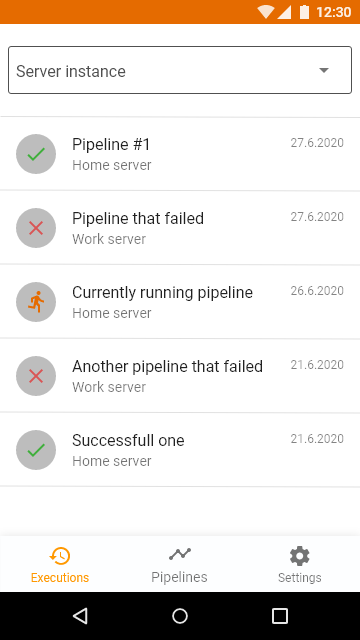
\includegraphics[width=\textwidth]{pics/xd/Bottom Navigation - executions.png}
    	\caption[History]{History screen design}\label{fig:xdHistory}
    \end{minipage}
    \begin{minipage}[b]{0.32\textwidth}
    	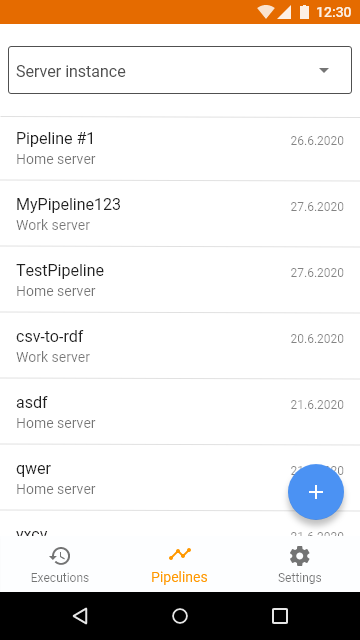
\includegraphics[width=\textwidth]{pics/xd/Bottom Navigation - pipelines.png}
    	\caption[Pipelines]{Pipelines screen design}\label{fig:xdPipelines}
    \end{minipage}
    \begin{minipage}[b]{0.32\textwidth}
    	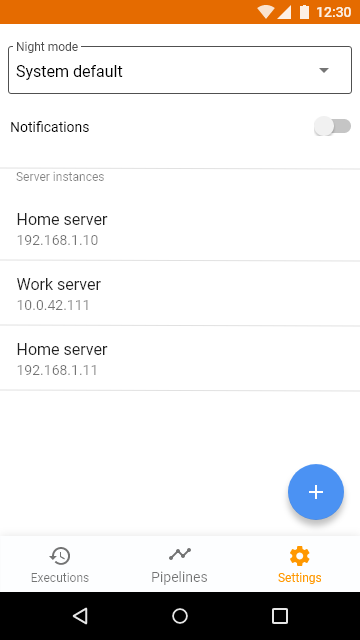
\includegraphics[width=\textwidth]{pics/xd/Bottom Navigation - settings.png}
    	\caption[Settings]{Settings screen design}\label{fig:xdSettings}
    \end{minipage}
\end{figure}

\section{Lists}
Each of the three main screens will display some sort of list.
For the execution screen it is a list of executions, for the pipeline screen it is a list of pipelines and for the settings screen it is a list of server instances.

All of those lists will have one thing in common and that being the swipe gesture.
When users swipe an item to the left or to the right, the item will be deleted.
This can be seen in \autoref{fig:xdDeletePipeline}.
Users will have the ability to undo this operation for a short period of time.
The undo option can be seen in \autoref{fig:xdUndo}.

Tapping on an item from the pipeline screen will open the edit pipeline screen.
Long click on item from execution screen or from pipeline screen will launch the pipeline.

\begin{figure}\centering
    \begin{minipage}[b]{0.32\textwidth}
    	\includegraphics[width=\textwidth]{pics/xd/Bottom Navigation - pipelines – 1.png}
    	\caption[Deleting pipeline]{Deleting pipeline design}\label{fig:xdDeletePipeline}
    \end{minipage}
    \begin{minipage}[b]{0.32\textwidth}
    	\includegraphics[width=\textwidth]{pics/xd/Bottom Navigation - pipelines – 2.png}
    	\caption[Undo option]{Undo option design}\label{fig:xdUndo}
    \end{minipage}
\end{figure}

\section{Edit server instance screen}
While registering a new server instance or editing an already registered one, the application needs the address for communication and some name for labeling and better organising.
Users will be able to add a description of the instance, so that there is no pressure to store every information about the instance in the server name.
There could also be an option to ping the server (F-2.6, \autoref{subsec:ping}) to verify the address and a way to cancel the registration/edit.
Because of this, another screen, just for registering/editing server instances, will be added and can be seen in \autoref{fig:xdEditServerInstance}.

\begin{figure}\centering
    \begin{minipage}[b]{0.32\textwidth}
    	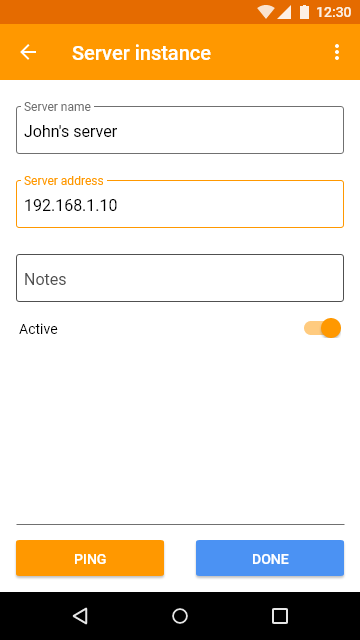
\includegraphics[width=\textwidth]{pics/xd/Edit server instance.png}
    	\caption[Edit server instance]{Edit server instance screen design}\label{fig:xdEditServerInstance}
    \end{minipage}
    \begin{minipage}[b]{0.32\textwidth}
    	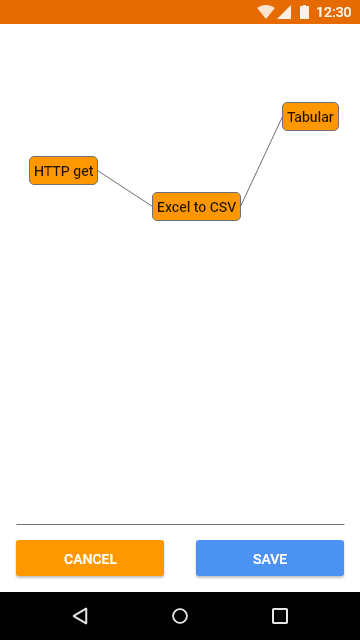
\includegraphics[width=\textwidth]{pics/xd/Pipeline editor.png}
    	\caption[Edit pipeline screen]{Edit pipeline screen design}\label{fig:xdPipelineEditor}
    \end{minipage}
\end{figure}

\section{Edit pipeline screen}
According to the F-4.3 requirement, described in \autoref{subsec:editpipelinescreen}, there has to be a screen for editing pipelines.
This screen will be displaying pipeline components and drawing links between them.
The preliminary design of this screen can be seen in \autoref{fig:xdPipelineEditor}

% \begin{figure}\centering
%     \begin{minipage}[b]{0.32\textwidth}
%     	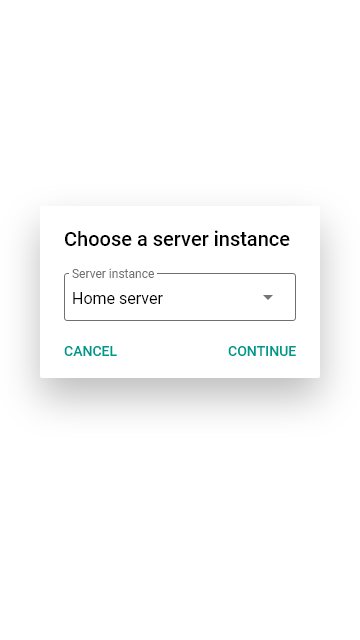
\includegraphics[width=\textwidth]{pics/xd/Create new pipeline.png}
%     	\caption[Create new pipeline dialog]{Create new pipeline dialog design}\label{fig:xdCreateNewPipelineDialog}
%     \end{minipage}
%     \begin{minipage}[b]{0.32\textwidth}
%     	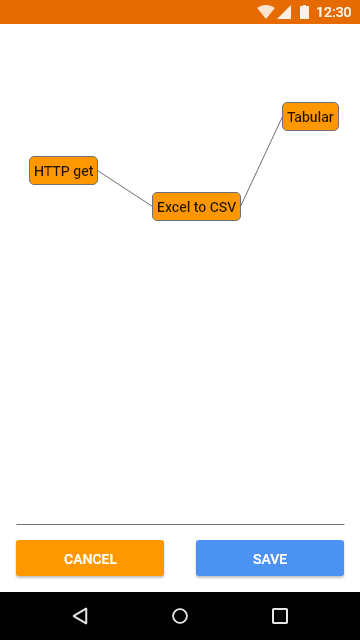
\includegraphics[width=\textwidth]{pics/xd/Pipeline editor.png}
%     	\caption[Edit pipeline screen]{Edit pipeline screen design}\label{fig:xdPipelineEditor}
%     \end{minipage}
% \end{figure}

\section{Edit component screen}
This screen has to be created, because each pipeline's component has its own settings.
In \autoref{fig:xdEditComponent1} and \autoref{fig:xdEditComponent2} is the preliminary design of this screen.

\begin{figure}\centering
    \begin{minipage}[b]{0.32\textwidth}
    	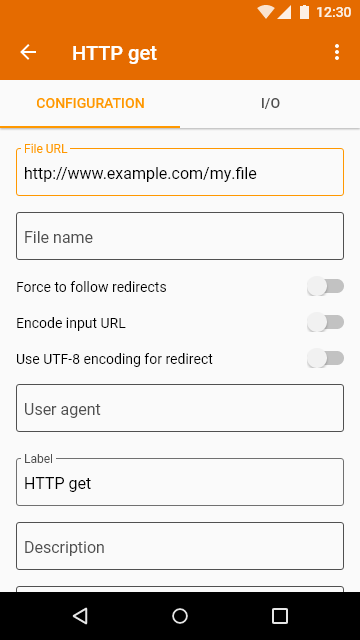
\includegraphics[width=\textwidth]{pics/xd/Edit component - configuration.png}
    	\caption[Edit component screen 1]{Edit component screen 1 design}\label{fig:xdEditComponent1}
    \end{minipage}
    \begin{minipage}[b]{0.32\textwidth}
    	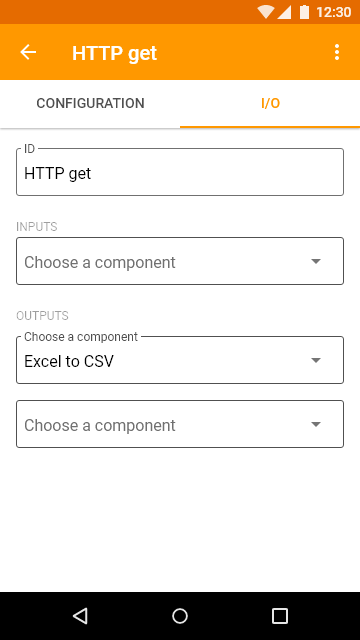
\includegraphics[width=\textwidth]{pics/xd/Edit component - io.png}
    	\caption[Edit component screen 2]{Edit component screen 2 design}\label{fig:xdEditComponent2}
    \end{minipage}
\end{figure}

\section{Notifications}
According to the F-3.1 requirement, described in \autoref{subsec:notifications}, notifications need to be implemented.
The preview of notifications can be seen in \autoref{fig:xdNotifications}.

\begin{figure}\centering
    \begin{minipage}[b]{0.7\textwidth}
    	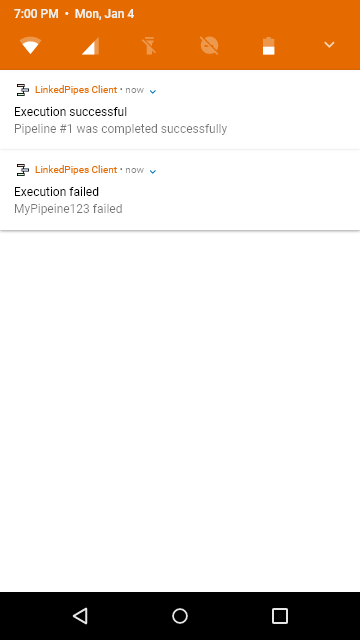
\includegraphics[width=\textwidth]{pics/xd/Notifications.png}
    	\caption[Notifications]{Notification design}\label{fig:xdNotifications}
    \end{minipage}
\end{figure}
% https://www.youtube.com/watch?v=ugpC98LcNqA
% https://www.youtube.com/watch?v=QrbhPcbZv0I

\section{Software architecture patterns}
Every non trivial software project should follow some architecture design.
But why? You want your project to be always maintainable and expandable as much easily as possible.
You want to modularize it, so that you can just take one part and exchange it without the need of rewriting the whole project.
And for this reason, there are architecture patterns.
I will describe three of them and explain my conclusion.

All of these three patterns have one thing in common.
They structure code into three main layers.
The names of those layers are present in these pattern's names.

\subsection{MVC}

\begin{figure}\centering
	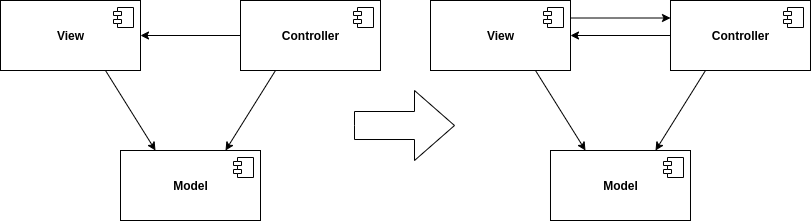
\includegraphics[width=1\textwidth]{pics/patterns/bc-mvc2.png}
	\caption[MVC]{Model View Controller}\label{fig:mvc}
\end{figure}

\textbf{Model View Controller}.
View is responsible for displaying data, controller is responsible for getting the user input and model for storing data.
The controller takes user input, it updates the model and then tells the view to update itself.

Now we know, that if we choose this, it will be implemented in android.
How does one do this? In the android world, the part of application responsible for displaying things is also responsible for dealing with user input.
So you tweak the pattern so the view gets the user input, it sends it to the controller, the controller updates the model, then tells the view to update itself, based on the data from model.

So both view and controller know the model, the view knows controller and controller knows view.
That's pretty bad, you don't want this.
That's high consistency and that is a thing you want to avoid, especially in the android world, where forgetting to remove a link can and will cause memory leaks.

And what if you want to somehow transform the data for presentation?
What part should do this presentation transformation, also known as UI logic?
You don't want to push this to the view, because you want the UI logic also to be easily testable and you want to separate it from the appearance of the view.
Controller can not posses it neither, because it doesn't supply any data to the view. So should you put it in the model? Absolutely not!
Why should a part of the application, responsible for data storing, know how to display stuff?

\subsection{MVP}

\begin{figure}\centering
	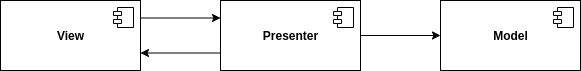
\includegraphics[width=0.7\textwidth]{pics/patterns/bc-mvp.png}
	\caption[MVP]{Model View Presenter}\label{fig:mvp}
\end{figure}

Imagine the MVC and the UI logic problem.
Now what if the view doesn't communicate with the model, but only with controller and the controller was also responsible for taking data from the model and supplying them to the view.
Then you would be able to put UI logic to this new controller. Now we will call it presenter, instead of new controller.
And that's what \textbf{Model View Presenter} is.

But that means the presenter still holds a link to the view. You still need to write some repetitive code because of this.
Second, why would the presenter should know, what parts of the view should be updated after the data changes?

\subsection{MVVM}

\begin{figure}\centering
	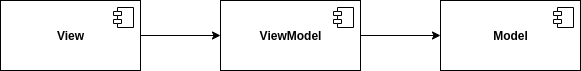
\includegraphics[width=0.7\textwidth]{pics/patterns/bc-mvvm.png}
	\caption[MVVM]{Model View ViewModel}\label{fig:mvvm}
\end{figure}

\textbf{Model View Viewmodel}.
We will borrow the MVP and tweak it a little. Currently the presenter knows the view and is executing it's methods when it needs to be updated.
Let's rename presenter to viewmodel. It no longer knows it's view.
Instead it provides some kind of stream and the view can observe the stream, so it can do whatever whenever it omits any data.

So the view knows the viewmodel, can call it's methods on user input and observe it's data streams.
The viewmodel knows model, observes it's data streams and omits them to the view.
The view knows the viewmodel, the viewmodel knows the model and the model don't know any of them.

\subsection{And the winner is ...}
Our choice is MVVM. Not only it looks like the tip of the evolution, but Google even made some libraries to support it.

\section{Main layers and libraries}
We will go over the three main layers of the MVVM, add a fourth at the end and describe some libraries that will be used inside of them.

\subsection{View}
As I said before, the view is the layer responsible for displaying data. It's what I call a screen in functional requirements.
The way it's implemented is through a combination of standard kotlin code and xml.
The xml is like a skeleton and kotlin is like life. In xml, you specify the look and in kotlin, you can specify what data it should display, how to update itself and what to do with user input.

For that, you have to somehow link or bind these two things (xml and kotlin) together.
We will be using a library called Data Binding. It's better than nothing and compared to other solutions, like kotlin's synthetics, Data Binding offers more features and I personally think it looks clearer.

\subsection{Viewmodel}
Google has made some architecture components and one of them is exactly for viewmodel.
It will be shame not to use it.

\subsection{Repository}
Repository will represent the model.
It's a place responsible for maintaining data.
Does the application need to download them, or load from cache?
Do you need to get anything out of the application or get anything in it?
You will ask the repository, also known as the one and the only source of truth.

\subsection{DAO and network IO}
This will be the fourth layer.
Every android app can run it's own SQLite database.
Data Access Objects will be used to access data in in this database.
There is a nice library for that called Room and we will be using it.
Network IO layer will be responsible for communication with server instance API.
We will be using Retrofit library for those API requests.
Repository will be using both of those in order to maintain and organise data.

\subsection{LiveData}
LiveData is a library.
It will be used in each layer.
Previously I talked about observing some kind of stream.
For this, you need some kind of observable variables and that's what LiveData is.
It enables you to set some action to happen when the data changes.
LiveData is not just some ordinary stream, it only streams, when there is some observer living.
It may sound silly, but for example, you don't need to update certain screen, when that screen is not visible.

\section{Conclusion}

\begin{figure}\centering
	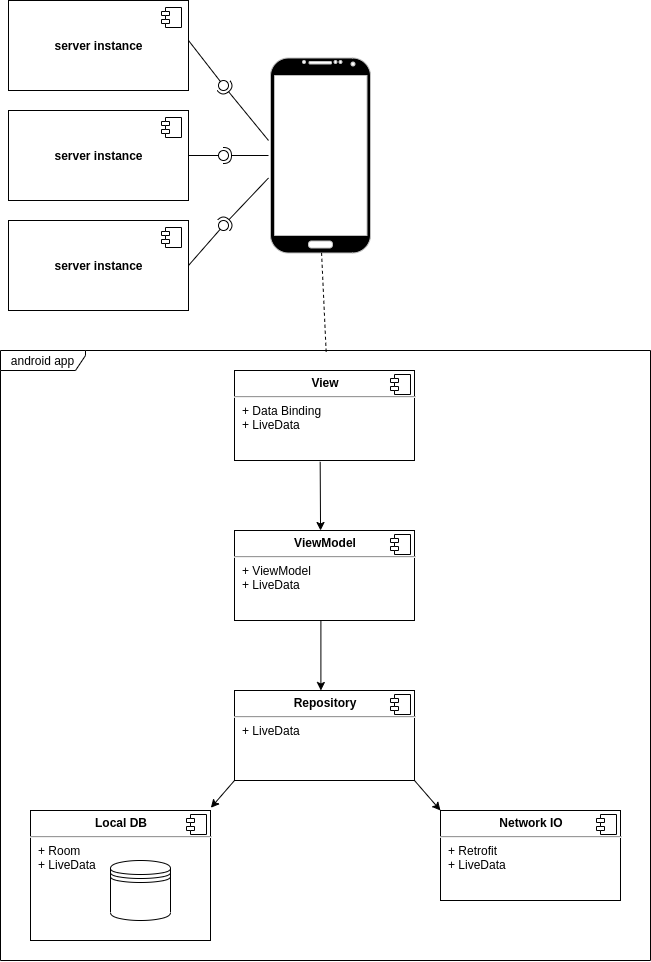
\includegraphics[width=1\textwidth]{pics/bc-architecture.png}
	\caption[Architecture]{Diagram consisting of MVVM and server instances}\label{fig:architecture}
\end{figure}

For better perspective, here is a summarizing diagram: \ref{fig:architecture}

The android device will communicate directly with multiple server instances. Network IO layer will be responsible for this communication. Repository will cache it using the Local DB layer and hand out data to the viewmodel. Viewmodel can do any UI logic that's needed and pass it to the view. All handing out or passing from any bottom layer to the one on top will be done through the observation of LiveData.

%\chapter{Realization}
\chapter{Implementation}
//TODO

\chapter{Deployment}
//TODO

\begin{conclusion}
	%sem napište závěr Vaší práce
	//TODO
\end{conclusion}

\bibliographystyle{csn690}
\bibliography{mybibliographyfile}

\appendix

\chapter{Seznam použitých zkratek}
% \printglossaries
\begin{description}
	\item[GUI] Graphical user interface
	\item[XML] Extensible markup language
	\item[Managing] Adding, editing, deleting
\item[Pipeline] A set of tasks defined in ETL LinkedPipes server instance
\item[Server instance] ETL LinkedPipes server instance
\item[User] Common user of the android application
\item[History] History of pipeline executions
\end{description}

\chapter{Obsah přiloženého CD}

%upravte podle skutecnosti

\begin{figure}
	\dirtree{%
		.1 readme.txt\DTcomment{stručný popis obsahu CD}.
		.1 exe\DTcomment{adresář se spustitelnou formou implementace}.
		.1 src.
		.2 impl\DTcomment{zdrojové kódy implementace}.
		.2 thesis\DTcomment{zdrojová forma práce ve formátu \LaTeX{}}.
		.1 text\DTcomment{text práce}.
		.2 thesis.pdf\DTcomment{text práce ve formátu PDF}.
		.2 thesis.ps\DTcomment{text práce ve formátu PS}.
	}
\end{figure}

\end{document}
